\section{Durchführung}
\label{sec:Durchführung}

\begin{figure}
    \centering
    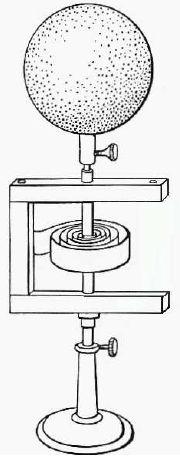
\includegraphics[height=6cm]{data/Bild_1}
    \caption{Aufbau}
    \label{fig:aufbau}
\end{figure}

Der grundlegende Aufbau ist in der kompletten Versuchsreihe gleichbleibend. Auf die Halterung, auf die im Bild\ref{fig:aufbau} die Kugel
montiert ist, werden im Folgenden alle zu untersuchenden Körper befestigt. 

\subsection{Bestimmung der Winkelrichtgröße $D$}

Um die Winkelrichtgröße $D$ zu bestimmen, wird unter die Halterung für den Körper eine Scheibe gelegt, auf der der Auslenkungswinkel 
abgelesen werden kann. In die Halterung wird anstelle der Kugel eine Stange waagerecht befestigt, die in deren Mitte verschraubt wird.
die Stange hat einen Durchmesser von 0,5$\si{\centi\meter}$ und ist 60$\si{\centi\meter}$ lang. An dieser wird 10$\si{\centi\meter}$
von der Drehachse entfernt ein Newtonmeter angebracht, welches immer senkrecht zur Stange ausgerichtet ist. An dem Newtonmeter 
angreifend wird die Stange ausgelenkt. Dies wird in 10$\si{\degree}$-Schritten von 20$\si{\degree}$ bis 90$\si{\degree}$ gemacht.
Dabei wird jeweils die wirkende Kraft notiert, die bei der bestimmten Auslenkung wirkt. 

\subsection{Bestimmung des Eigenträgheitsmoments}

Hierbei wird die selbe Stange verwendet. auf beiden Seiten wird jeweils eine Masse $m=223,3\si{\gram}$ in gleichem Abstand zur 
Drehachse montiert. Die Stange wird dann um einen kleinen Winkel ausgelenkt und losgelassen. Es wird die Periodendauer der Schwingung
mit einer Stoppuhr gemessen und notiert. Der Versuch wird mit zehn unterschiedlichen Abständen der Gewichte zur Drehachse durchgeführt.

\subsection{Bestimmung unterschiedlicher Trägheitsmomente}



